% Shared preamble and macros of the method figure v3 candidates (method_v3a.tex, method_v3b.tex) and the chosen
% method_v3.tex. Data assets: fig_method_v3.py writes ../method_v3/ (thumbnails, reach-table cards, data.tex with
% the three quadratics of panel (c)). Units: 1 unit = 1 pt at print size (5.5 in = 397.48 pt wide).
% Text: titles 9 pt bold sans, labels 7.5 pt, small labels 7 pt; math 8 pt (scripts 6 pt). Palette: sca_colors.tex
% (green SCA, amber local window, blue global grid, greys).
\documentclass[border=0pt]{standalone}
\RequirePackage{fix-cm}
\usepackage[T1]{fontenc}
\usepackage{helvet}
\usepackage{amsmath}
\usepackage{graphicx}
\usepackage{tikz}
\usetikzlibrary{arrows.meta, calc}
\DeclareMathSizes{7}{7}{6}{6}
\DeclareMathSizes{7.5}{7.5}{6}{6}
\DeclareMathSizes{8}{8}{6.2}{6}
\DeclareMathSizes{8.5}{8.5}{6.5}{6}
\DeclareMathSizes{9}{9}{6.5}{6}
\DeclareMathSizes{10}{10}{7}{6}
% Written by scafig.py; the same palette as the matplotlib figures.
\definecolor{scaInk}{HTML}{1F2328}
\definecolor{scaMid}{HTML}{5B6570}
\definecolor{scaRule}{HTML}{C3C9CF}
\definecolor{scaGrid}{HTML}{E6E9EC}
\definecolor{scaGlobal}{HTML}{2F6DB3}
\definecolor{scaGlobalLight}{HTML}{DCE7F3}
\definecolor{scaLocal}{HTML}{E08A2B}
\definecolor{scaLocalLight}{HTML}{F9E6D0}
\definecolor{scaAccent}{HTML}{13865F}
\definecolor{scaAccentLight}{HTML}{D7EEE4}
\definecolor{scaNeutral}{HTML}{F4F1EA}
\definecolor{scaZoom}{HTML}{FFC21A}
\definecolor{scaLoss}{HTML}{B85C00}
\definecolor{scaArea}{HTML}{7A4EA3}
\definecolor{scaAreaLight}{HTML}{E9E0F1}
\definecolor{scaFull}{HTML}{9AA3AC}
\definecolor{scaCrop}{HTML}{E4572E}

% Written by fig_method_v3.py from results/evidence/calib/k1_1024.npz; do not edit by hand.
% Block 12, sigma bin centred at 0.618, ratio 4; J rescaled to [0, 1] over pi in [0, 1] per head.
% head 7: B/A = -0.185, pi* = 0.000
\def\JcG{(0.000,0.0000) (0.025,0.0072) (0.050,0.0154) (0.075,0.0244) (0.100,0.0343) (0.125,0.0452) (0.150,0.0570) (0.175,0.0697) (0.200,0.0833) (0.225,0.0978) (0.250,0.1132) (0.275,0.1296) (0.300,0.1468) (0.325,0.1650) (0.350,0.1840) (0.375,0.2040) (0.400,0.2249) (0.425,0.2467) (0.450,0.2695) (0.475,0.2931) (0.500,0.3176) (0.525,0.3431) (0.550,0.3695) (0.575,0.3967) (0.600,0.4249) (0.625,0.4540) (0.650,0.4840) (0.675,0.5150) (0.700,0.5468) (0.725,0.5796) (0.750,0.6132) (0.775,0.6478) (0.800,0.6833) (0.825,0.7197) (0.850,0.7570) (0.875,0.7952) (0.900,0.8343) (0.925,0.8744) (0.950,0.9154) (0.975,0.9572) (1.000,1.0000)}
\def\JpG{0.000}
% head 14: B/A = 0.749, pi* = 0.749
\def\JcM{(0.000,1.0000) (0.025,0.9343) (0.050,0.8709) (0.075,0.8097) (0.100,0.7508) (0.125,0.6940) (0.150,0.6395) (0.175,0.5872) (0.200,0.5372) (0.225,0.4894) (0.250,0.4438) (0.275,0.4004) (0.300,0.3593) (0.325,0.3204) (0.350,0.2837) (0.375,0.2493) (0.400,0.2170) (0.425,0.1870) (0.450,0.1593) (0.475,0.1338) (0.500,0.1105) (0.525,0.0894) (0.550,0.0705) (0.575,0.0539) (0.600,0.0395) (0.625,0.0274) (0.650,0.0174) (0.675,0.0097) (0.700,0.0043) (0.725,0.0010) (0.750,0.0000) (0.775,0.0012) (0.800,0.0047) (0.825,0.0103) (0.850,0.0182) (0.875,0.0284) (0.900,0.0407) (0.925,0.0553) (0.950,0.0721) (0.975,0.0912) (1.000,0.1124)}
\def\JpM{0.749}
% head 9: B/A = 1.017, pi* = 1.000
\def\JcL{(0.000,1.0000) (0.025,0.9514) (0.050,0.9041) (0.075,0.8579) (0.100,0.8130) (0.125,0.7692) (0.150,0.7267) (0.175,0.6854) (0.200,0.6453) (0.225,0.6064) (0.250,0.5687) (0.275,0.5322) (0.300,0.4969) (0.325,0.4629) (0.350,0.4300) (0.375,0.3984) (0.400,0.3679) (0.425,0.3387) (0.450,0.3107) (0.475,0.2839) (0.500,0.2582) (0.525,0.2339) (0.550,0.2107) (0.575,0.1887) (0.600,0.1679) (0.625,0.1484) (0.650,0.1300) (0.675,0.1129) (0.700,0.0969) (0.725,0.0822) (0.750,0.0687) (0.775,0.0564) (0.800,0.0453) (0.825,0.0354) (0.850,0.0267) (0.875,0.0192) (0.900,0.0130) (0.925,0.0079) (0.950,0.0041) (0.975,0.0014) (1.000,0.0000)}
\def\JpL{1.000}

\definecolor{scaLocalText}{HTML}{A85F12}
\definecolor{scaGlobalText}{HTML}{245A96}

\newcommand{\ttl}{\fontsize{9}{10.5}\selectfont\sffamily\bfseries}
\newcommand{\lab}{\fontsize{7.5}{9}\selectfont\sffamily}
\newcommand{\sml}{\fontsize{7}{8}\selectfont\sffamily}
\newcommand{\mth}{\fontsize{8}{9.5}\selectfont}
\newcommand{\mtb}{\fontsize{8.5}{10}\selectfont}
\newcommand{\mts}{\fontsize{7}{8}\selectfont}
\newcommand{\bigsym}{\fontsize{10}{12}\selectfont}

\tikzset{
  every node/.style={inner sep=0pt, outer sep=0pt, text=scaInk},
  arr/.style={-{Stealth[length=3.2pt, width=2.8pt]}, line width=0.6pt, draw=scaInk},
  blk/.style={rounded corners=2pt, line width=0.8pt},
  sblk/.style={blk, draw=scaAccent, fill=scaAccentLight},
  nblk/.style={blk, draw=scaFull, fill=white},
  axis/.style={line width=0.5pt, draw=scaMid},
}

% ---------------------------------------------------------------- the 1024^2 canvas (64 x 64 tokens, ratio 4)
% Window: 16 x 16 tokens, rows 19..34 and columns 23..38 (row 0 at the top), centred on the query tile;
% query tile drawn enlarged to 4 x 4 tokens (rows 25..28, columns 29..32); block centres at 4b + 2, b = 0..15.
\newcommand{\WinBox}[1]{(23*#1/64,{#1-35*#1/64}) rectangle (39*#1/64,{#1-19*#1/64})}
\newcommand{\Query}[1]{%
  \fill[scaInk] (29*#1/64,{#1-29*#1/64}) rectangle (33*#1/64,{#1-25*#1/64});
  \draw[white, line width=0.35pt] (29*#1/64,{#1-29*#1/64}) rectangle (33*#1/64,{#1-25*#1/64});}
% \Cv{x}{y}{side}{mode}: 0 full (all keys), 1 window (near set, local view), 2 outside the window (far set),
% 3 block-centre grid (global view).
\newcommand{\Cv}[4]{%
  \begin{scope}[shift={(#1,#2)}]
    \node[anchor=south west] at (0,0) {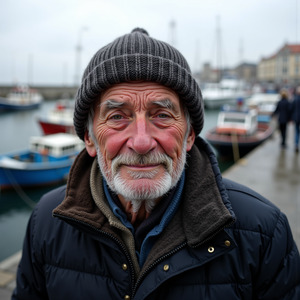
\includegraphics[width=#3pt]{../method_v3/canvas_1024.jpg}};
    \ifcase#4
    \or
      \fill[white, opacity=0.68, even odd rule] (0,0) rectangle (#3,#3) \WinBox{#3};
      \draw[line width=0.9pt, scaLocal] \WinBox{#3};
    \or
      \fill[white, opacity=0.80] \WinBox{#3};
      \draw[line width=0.6pt, scaLocal, dash pattern=on 1.3pt off 0.9pt] \WinBox{#3};
    \or
      \fill[white, opacity=0.6] (0,0) rectangle (#3,#3);
      \foreach \i in {0,...,15}{\foreach \j in {0,...,15}{
        \fill[scaGlobal] ({(4*\i+2.5)*#3/64},{#3-(4*\j+2.5)*#3/64}) circle[radius=0.42pt];}}
    \fi
    \draw[line width=0.6pt, scaFull] (0,0) rectangle (#3,#3);
    \Query{#3}
  \end{scope}}

% ---------------------------------------------------------------- the 4096^2 target (256 x 256 tokens)
% Native window of 64 tokens, rows 144..207 and columns 124..187, centred on the query tile (rows 172..179,
% columns 152..159, on a sheep); block centres every 4 tokens (64 x 64), drawn to scale.
\newcommand{\TgWin}[1]{(124*#1/256,{#1-208*#1/256}) rectangle (188*#1/256,{#1-144*#1/256})}
\newcommand{\Tg}[3]{% x y side
  \begin{scope}[shift={(#1,#2)}]
    \node[anchor=south west] at (0,0) {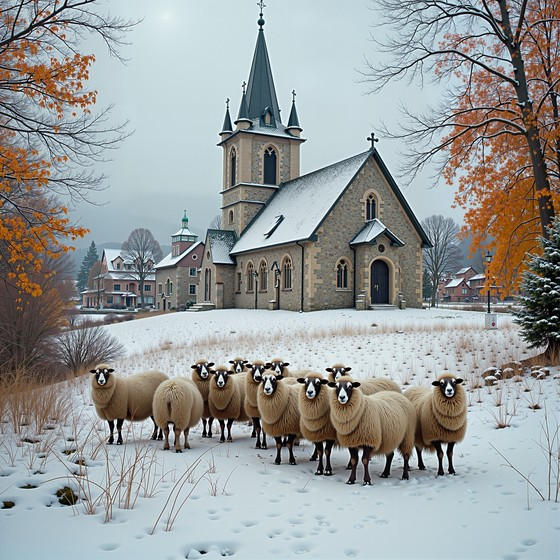
\includegraphics[width=#3pt]{../method_v3/target_4096.jpg}};
    \fill[white, opacity=0.55] (0,0) rectangle (#3,#3);
    \foreach \i in {0,...,63}{\foreach \j in {0,...,63}{
      \fill[scaGlobal] ({(4*\i+2.5)*#3/256},{#3-(4*\j+2.5)*#3/256}) circle[radius=0.17pt];}}
    \draw[line width=0.9pt, scaLocal] \TgWin{#3};
    \draw[line width=0.6pt, scaFull] (0,0) rectangle (#3,#3);
    \fill[scaInk] (152*#3/256,{#3-180*#3/256}) rectangle (160*#3/256,{#3-172*#3/256});
  \end{scope}}
% The same two views on the 1024^2 canvas at ratio 4 (window 16, grid 16 x 16), for the emulation mapping.
\newcommand{\Em}[3]{% x y side
  \begin{scope}[shift={(#1,#2)}]
    \node[anchor=south west] at (0,0) {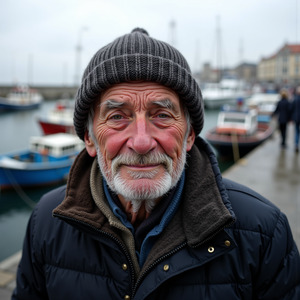
\includegraphics[width=#3pt]{../method_v3/canvas_1024.jpg}};
    \fill[white, opacity=0.55] (0,0) rectangle (#3,#3);
    \foreach \i in {0,...,15}{\foreach \j in {0,...,15}{
      \fill[scaGlobal] ({(4*\i+2.5)*#3/64},{#3-(4*\j+2.5)*#3/64}) circle[radius=0.3pt];}}
    \draw[line width=0.9pt, scaLocal] \WinBox{#3};
    \draw[line width=0.6pt, scaFull] (0,0) rectangle (#3,#3);
    \Query{#3}
  \end{scope}}

% ---------------------------------------------------------------- panel (c): three quadratics J(pi)
% \Quad{x0}{y0}{w}{h}: box with the three rescaled curves of data.tex and their minimizers pi* = clip(B/A, 0, 1);
% y maps [-0.08, 1.04] to the box so that the minima sit just above the axis.
\newcommand{\Quad}[4]{%
  \begin{scope}[shift={(#1,#2)}]
    \begin{scope}[xscale=#3, yscale=#4/1.12, shift={(0,0.08)}]
      \draw[line width=0.9pt, scaGlobal, line join=round] plot coordinates {\JcG};
      \draw[line width=0.9pt, scaInk, line join=round] plot coordinates {\JcM};
      \draw[line width=0.9pt, scaLocal, line join=round] plot coordinates {\JcL};
    \end{scope}
    \draw[axis] (0,0) -- (#3,0);
    \draw[axis] (0,0) -- (0,#4);
    \foreach \p in {\JpG,\JpM,\JpL}{
      \fill[scaAccent] ({#3*\p},{#4*0.08/1.12}) circle[radius=1.5pt];}
    \draw[scaMid, line width=0.4pt, dash pattern=on 1pt off 1pt] ({#3*\JpM},{#4*0.08/1.12}) -- ({#3*\JpM},0);
    \foreach \v/\t in {0/0, 1/1}{
      \draw[axis] ({#3*\v},0) -- ({#3*\v},-1.6);
      \node[anchor=north, text=scaMid] at ({#3*\v},-2.4) {\sml\t};}
    \node[anchor=north] at ({#3*\JpM},-2.0) {\mts$\pi^\star$};
    \node[anchor=west, text=scaMid] at (#3+2,0) {\mth$\pi$};
    \node[anchor=east, text=scaMid] at (-2,#4-3) {\mth$J$};
  \end{scope}}

% ---------------------------------------------------------------- panel (d): schematic views at a stage
\newcommand{\Tile}[1]{\fill[scaGrid] (0,0) rectangle (#1,#1); \draw[line width=0.5pt, scaFull] (0,0) rectangle (#1,#1);}
\newcommand{\QueryC}[1]{\fill[scaInk] ({0.47*#1},{0.53*#1}) rectangle ++({0.07*#1},{0.07*#1});
  \draw[white, line width=0.3pt] ({0.47*#1},{0.53*#1}) rectangle ++({0.07*#1},{0.07*#1});}
\newcommand{\LocIcon}[4]{\begin{scope}[shift={(#1,#2)}]\Tile{#3}
  \pgfmathsetmacro{\wh}{0.5*#3/#4}
  \fill[scaLocalLight] ({0.505*#3-\wh},{0.565*#3-\wh}) rectangle ({0.505*#3+\wh},{0.565*#3+\wh});
  \draw[scaLocal, line width=0.8pt] ({0.505*#3-\wh},{0.565*#3-\wh}) rectangle ({0.505*#3+\wh},{0.565*#3+\wh});
  \QueryC{#3}\end{scope}}
\newcommand{\GlobIcon}[4]{\begin{scope}[shift={(#1,#2)}]\Tile{#3}
  \foreach \i in {0,...,11}{\foreach \j in {0,...,11}{\fill[scaGlobal] ({(\i+0.5)*#3/12},{(\j+0.5)*#3/12}) circle[radius=0.42pt];}}
  \QueryC{#3}\end{scope}}
% One SCA stage: green block holding the per-head mix at ratio #4; lower-left (#1,#2), width #3, height 30.
\newcommand{\SCAStage}[4]{\begin{scope}[shift={(#1,#2)}]
  \draw[sblk] (0,0) rectangle (#3,30);
  \node[anchor=east] at (17,15) {\mth $\pi_h$};
  \LocIcon{18.5}{4}{22}{#4}
  \node at (46.5,15) {\mth $+$};
  \node[anchor=east] at (84,15) {\mth $(1-\pi_h)$};
  \GlobIcon{85.5}{4}{22}{#4}
  \end{scope}}
% Reach-table cards (one block, 24 heads x 13 noise bins): ratio 2 behind, ratio 4 in front; lower-left of the
% front card (#1,#2), card size #3 x #4, offset 5.
\newcommand{\Cards}[4]{%
  \node[anchor=south west] at (#1+5,#2+5) {
\includegraphics[width=#3pt, height=#4pt]{../method_v3/table_r2.png}};
  \draw[line width=0.5pt, scaFull] (#1+5,#2+5) rectangle ++(#3,#4);
  \fill[white] (#1,#2) rectangle ++(#3,#4);
  \node[anchor=south west] at (#1,#2) {
\includegraphics[width=#3pt, height=#4pt]{../method_v3/table_r4.png}};
  \draw[line width=0.5pt, scaFull] (#1,#2) rectangle ++(#3,#4);}
